\subsection{Estudo puramente geométrico}
% Author: Renan
A abordagem puramente geométrica é uma análise do espaço de trabalho do
manipulador na pá. Utiliza os manipuladores da pesquisa de mercado como
objetos deste estudo e leva em consideração as dimensões da
pistola, o ângulo máximo e mínimo para o revestimento ($90^o \pm 60^o$), e a
distância mínima de 230 mm entre a pistola e a pá. É um estudo simplificado por não considerar as possíveis colisões com o ambiente, assumir
que a pá está contida em um plano (projeção, objeto 2D) e considerar o espaço
de trabalho do manipulador simétrico. A abordagem geométrica foi desenvolvida
com o auxílio do software Geogebra.

Primeiramente, o espaço de trabalho do manipulador é aproximado
como uma esfera, delimitada pelo espaço de
trabalho real do manipulador. A pá é projetada em planos, como mostra a
figura~\ref{fig::paplanos}, e, conforme o manipulador se aproxima da pá, o plano
direito corta a esfera (espaço de trabalho do manipulador). A interseção
entre o plano e a esfera é um círculo de raio $\overline{CB^i}$, que pode ser
calculado e estimado como a área revestida da pá. A distância ótima entre o
manipulador e a pá é calculada no limite em que o ângulo
$\overline{OB^iC}=30^o$. Finalmente, podem ser calculadas quantas posições
distintas o manipulador deve assumir para que toda a pá seja revestida, a partir
do modelo planar da pá e da turbina, figura~\ref{fig::pa2D}.

Essa abordagem é específica para cada manipulador da pesquisa de mercado.

\begin{figure}[h!]
	\centering	
	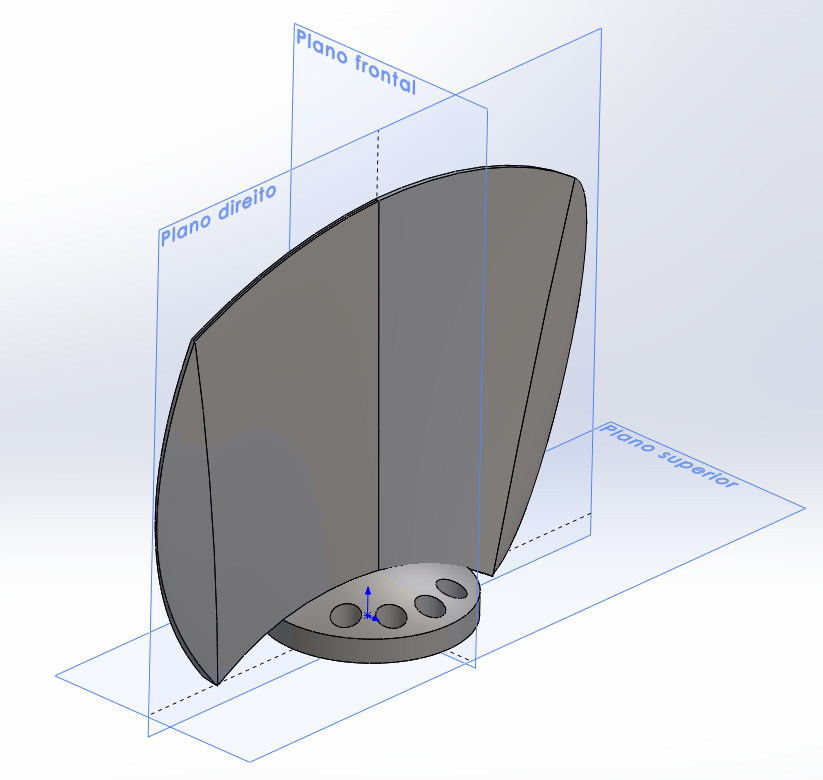
\includegraphics[width=0.6\columnwidth]{detail/figs/bighatch/PaPlanos.PNG}
	\caption{Ilustração das projeções da pá em planos.}
	\label{fig::paplanos}
\end{figure}

\begin{figure}[h!]
	\centering	
	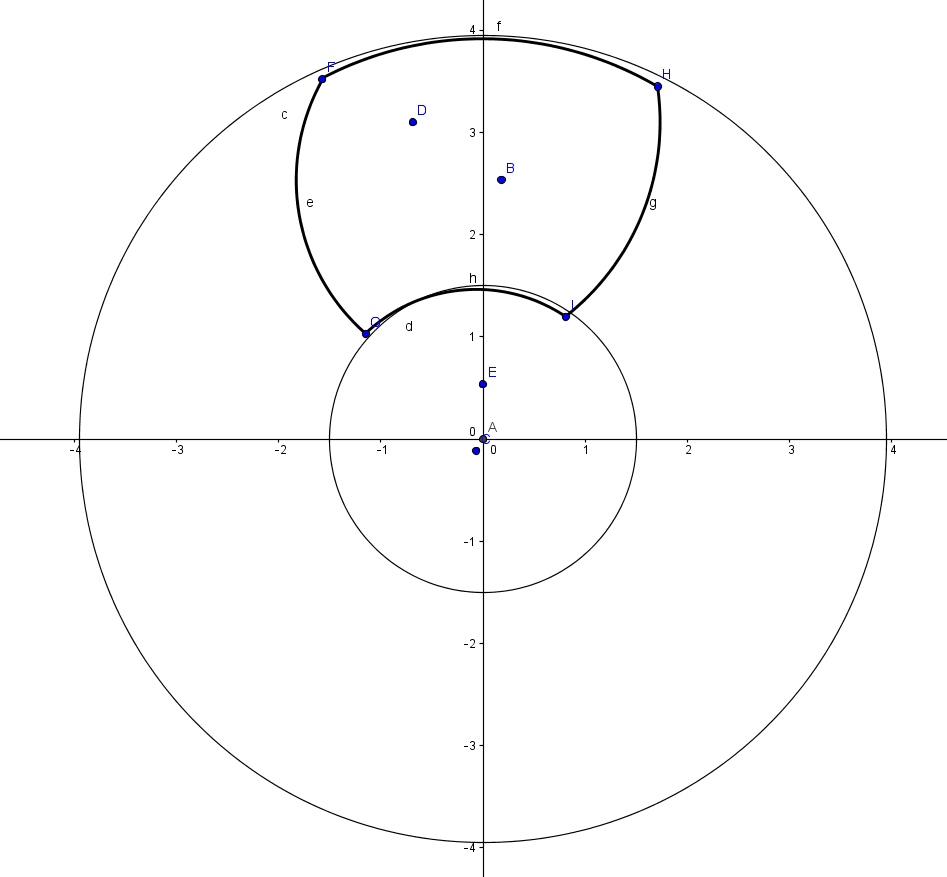
\includegraphics[width=0.6\columnwidth]{detail/figs/bighatch/pa2D.png}
	\caption{Ilustração do modelo 2D da pá.}
	\label{fig::pa2D}
\end{figure}

\paragraph{KR 10 R1100 sixx WP (Kuka)}
A figura~\ref{fig::kukageom} ilustra a interseção do espaço de trabalho
simplificado do manipulador Kuka KR10 e a projeção da pá. No
caso do Kuka KR 10 R1100, o raio da esfera é aproximado a $\overline{OB^i} = $
alcance do manipulador + comprimento da pistola + 230 mm. 

Para este manipulador, obtemos área revestida de $1.41^2\pi m^2$ e distância
ótima manipulador-pá de $0.82 m$. Dessa forma, são necessárias, pelo menos,
quatro posições distintas do manipulador a fim de toda a pá ser revestida. A
figura~\ref{fig::kukacircles} ilustra os pontos que o manipulador deve assumir
para revestir toda a pá. 

\begin{figure}[h!]
	\centering	
	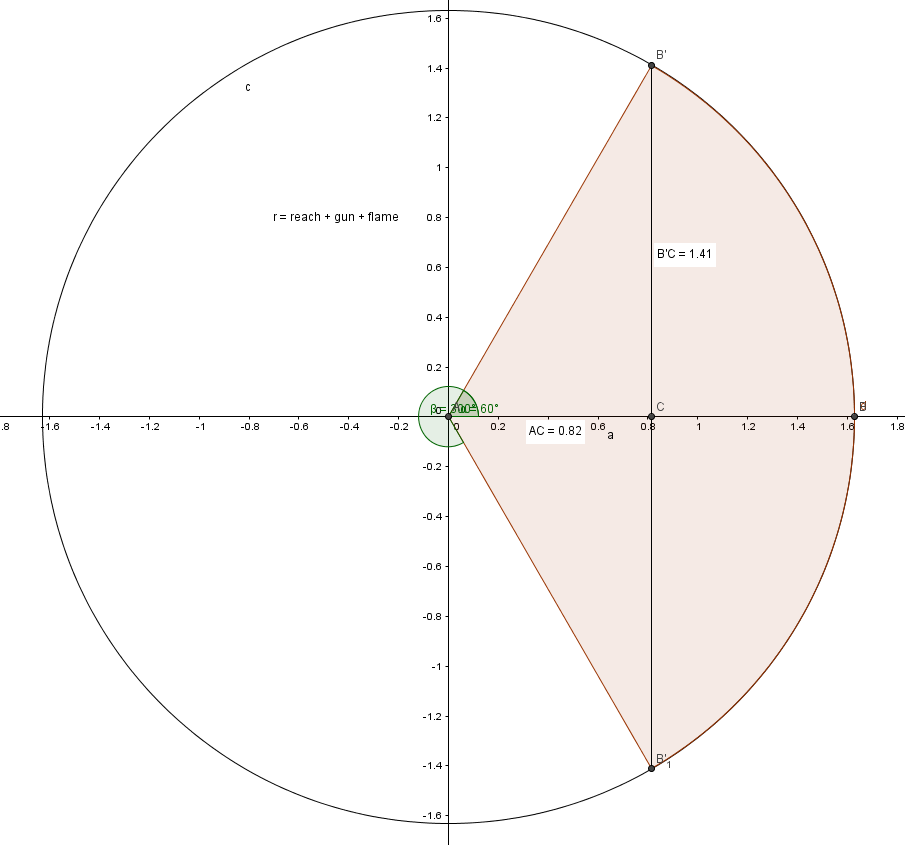
\includegraphics[width=0.6\columnwidth]{detail/figs/bighatch/kukageom.jpg}
	\caption{Ilustração da interseção do espaço de trabalho simplificado do
	manipulador Kuka KR10 e a projeção da pá.}
	\label{fig::kukageom}
\end{figure}

\begin{figure}[h!]	
	\centering
	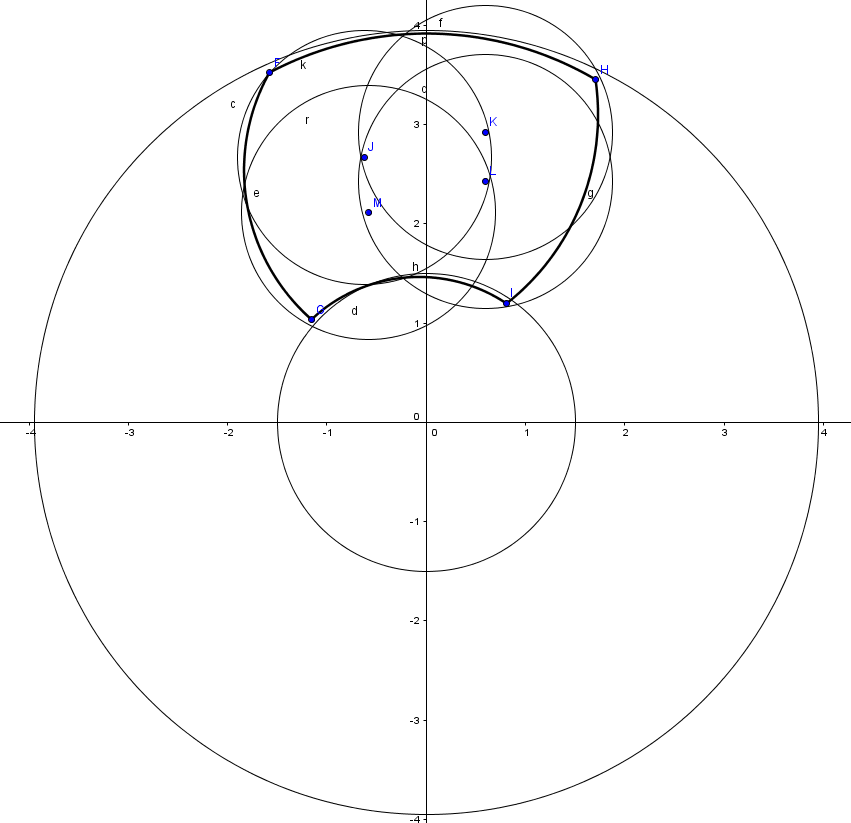
\includegraphics[width=0.6\columnwidth]{detail/figs/bighatch/kukacircles.png}
	\caption{Posições do manipulador Kuka KR10 para o processo de
	revestimento ser realizado em toda a pá.}
	\label{fig::kukacircles}
\end{figure}

\paragraph{MH12 (Motoman)}
A figura~\ref{fig::mh12geom} ilustra a interseção do espaço de trabalho
simplificado do manipulador MH12 e a projeção da pá. No
caso do MH12, o raio da esfera é aproximado a $\overline{OB^i} = $
alcance do manipulador + comprimento da pistola + 230 mm. 

Para este manipulador, obtemos área revestida de $1.54^2\pi m^2$ e distância
ótima manipulador-pá de $0.89 m$. Dessa forma, são necessárias, pelo menos,
duas posições distintas do manipulador a fim de toda a pá ser revestida. A
figura~\ref{fig::mh12circles} ilustra os pontos que o manipulador deve assumir
para revestir toda a pá.		

\begin{figure}[h!]	
	\centering
	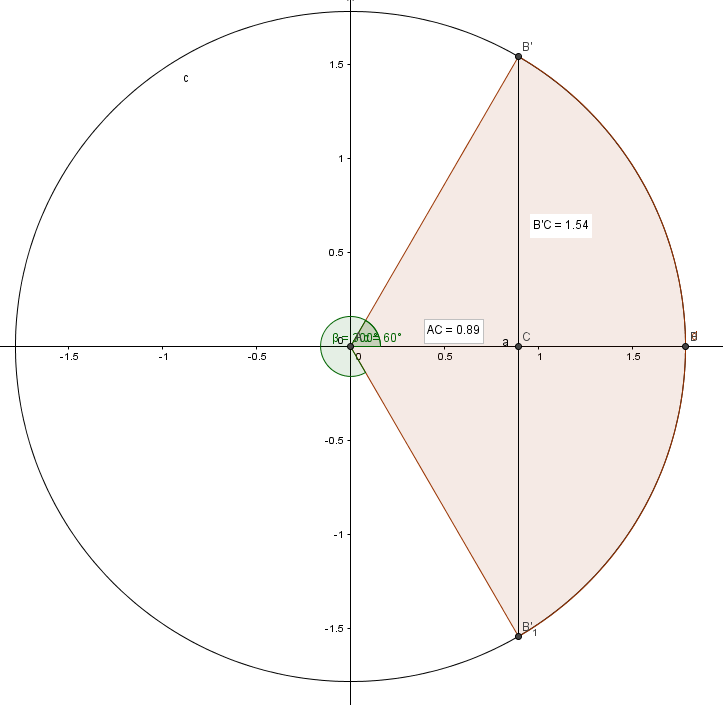
\includegraphics[width=0.6\columnwidth]{detail/figs/bighatch/mh12geom.jpg}
	\caption{Ilustração da interseção do espaço de trabalho simplificado do
	manipulador Motoman MH12 e a projeção da pá.}
	\label{fig::mh12geom}
\end{figure}

\begin{figure}[h!]	
	\centering
	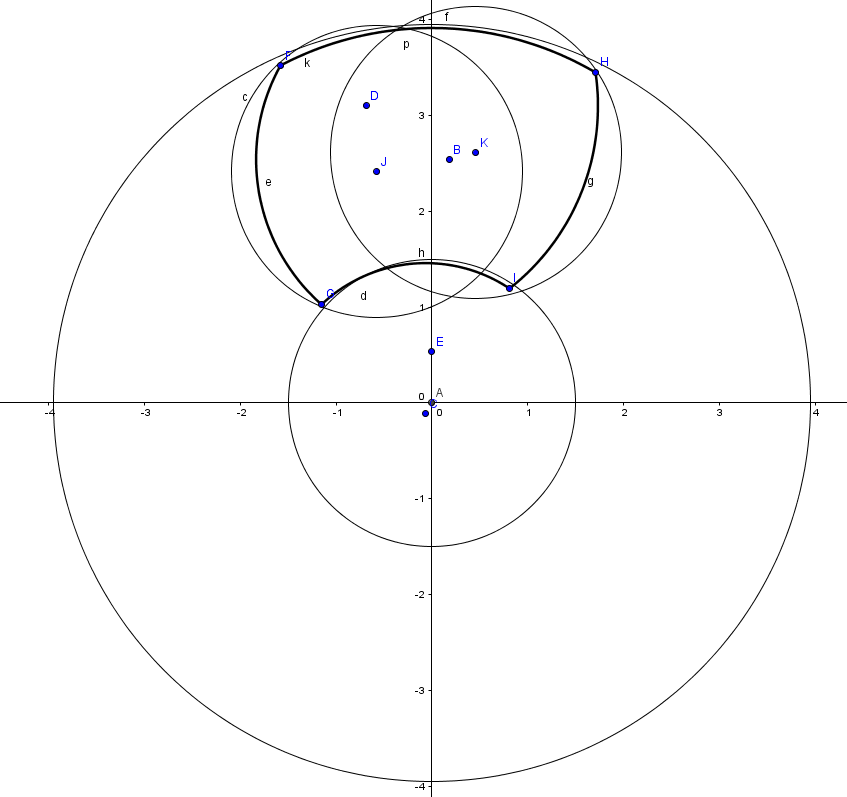
\includegraphics[width=0.6\columnwidth]{detail/figs/bighatch/mh12circles.png}
	\caption{Posições do manipulador MH12 para o processo de
	revestimento ser realizado em toda a pá.}
	\label{fig::mh12circles}
\end{figure}